%!TEX root = ../intro.tex
%******************************
%	 Sources of expression noise
%*****************************

\section{Sources of expression noise} 

Variability in expression across homogeneous populations of cells arises from intrinsic and extrinsic noise (see \textbf{Box 1}). While intrinsic noise is promoter-specific and therefore induces uncoordinated variation in RNA or protein expression between individual genes, extrinsic noise globally influences gene expression across multiple cells and therefore leads to co-variation across larger sets of genes. Here, I give an overview on the different sources of intrinsic and extrinsic noise in a variety of biological systems.

\subsection{Intrinsic noise}

Intrinsic noise in cell populations arises from stochasticity in biochemical reactions that leads to the synthesis of mRNAs (transcription) and proteins (translation) within individual cells. Regulatory features on the genomic, epigenetic, transcriptional and translational level influence the strength of intrinsic noise (for an overview see \textbf{Fig.~\ref{fig0:overview_intrinsic}}).

\begin{figure}[!h]
\centering
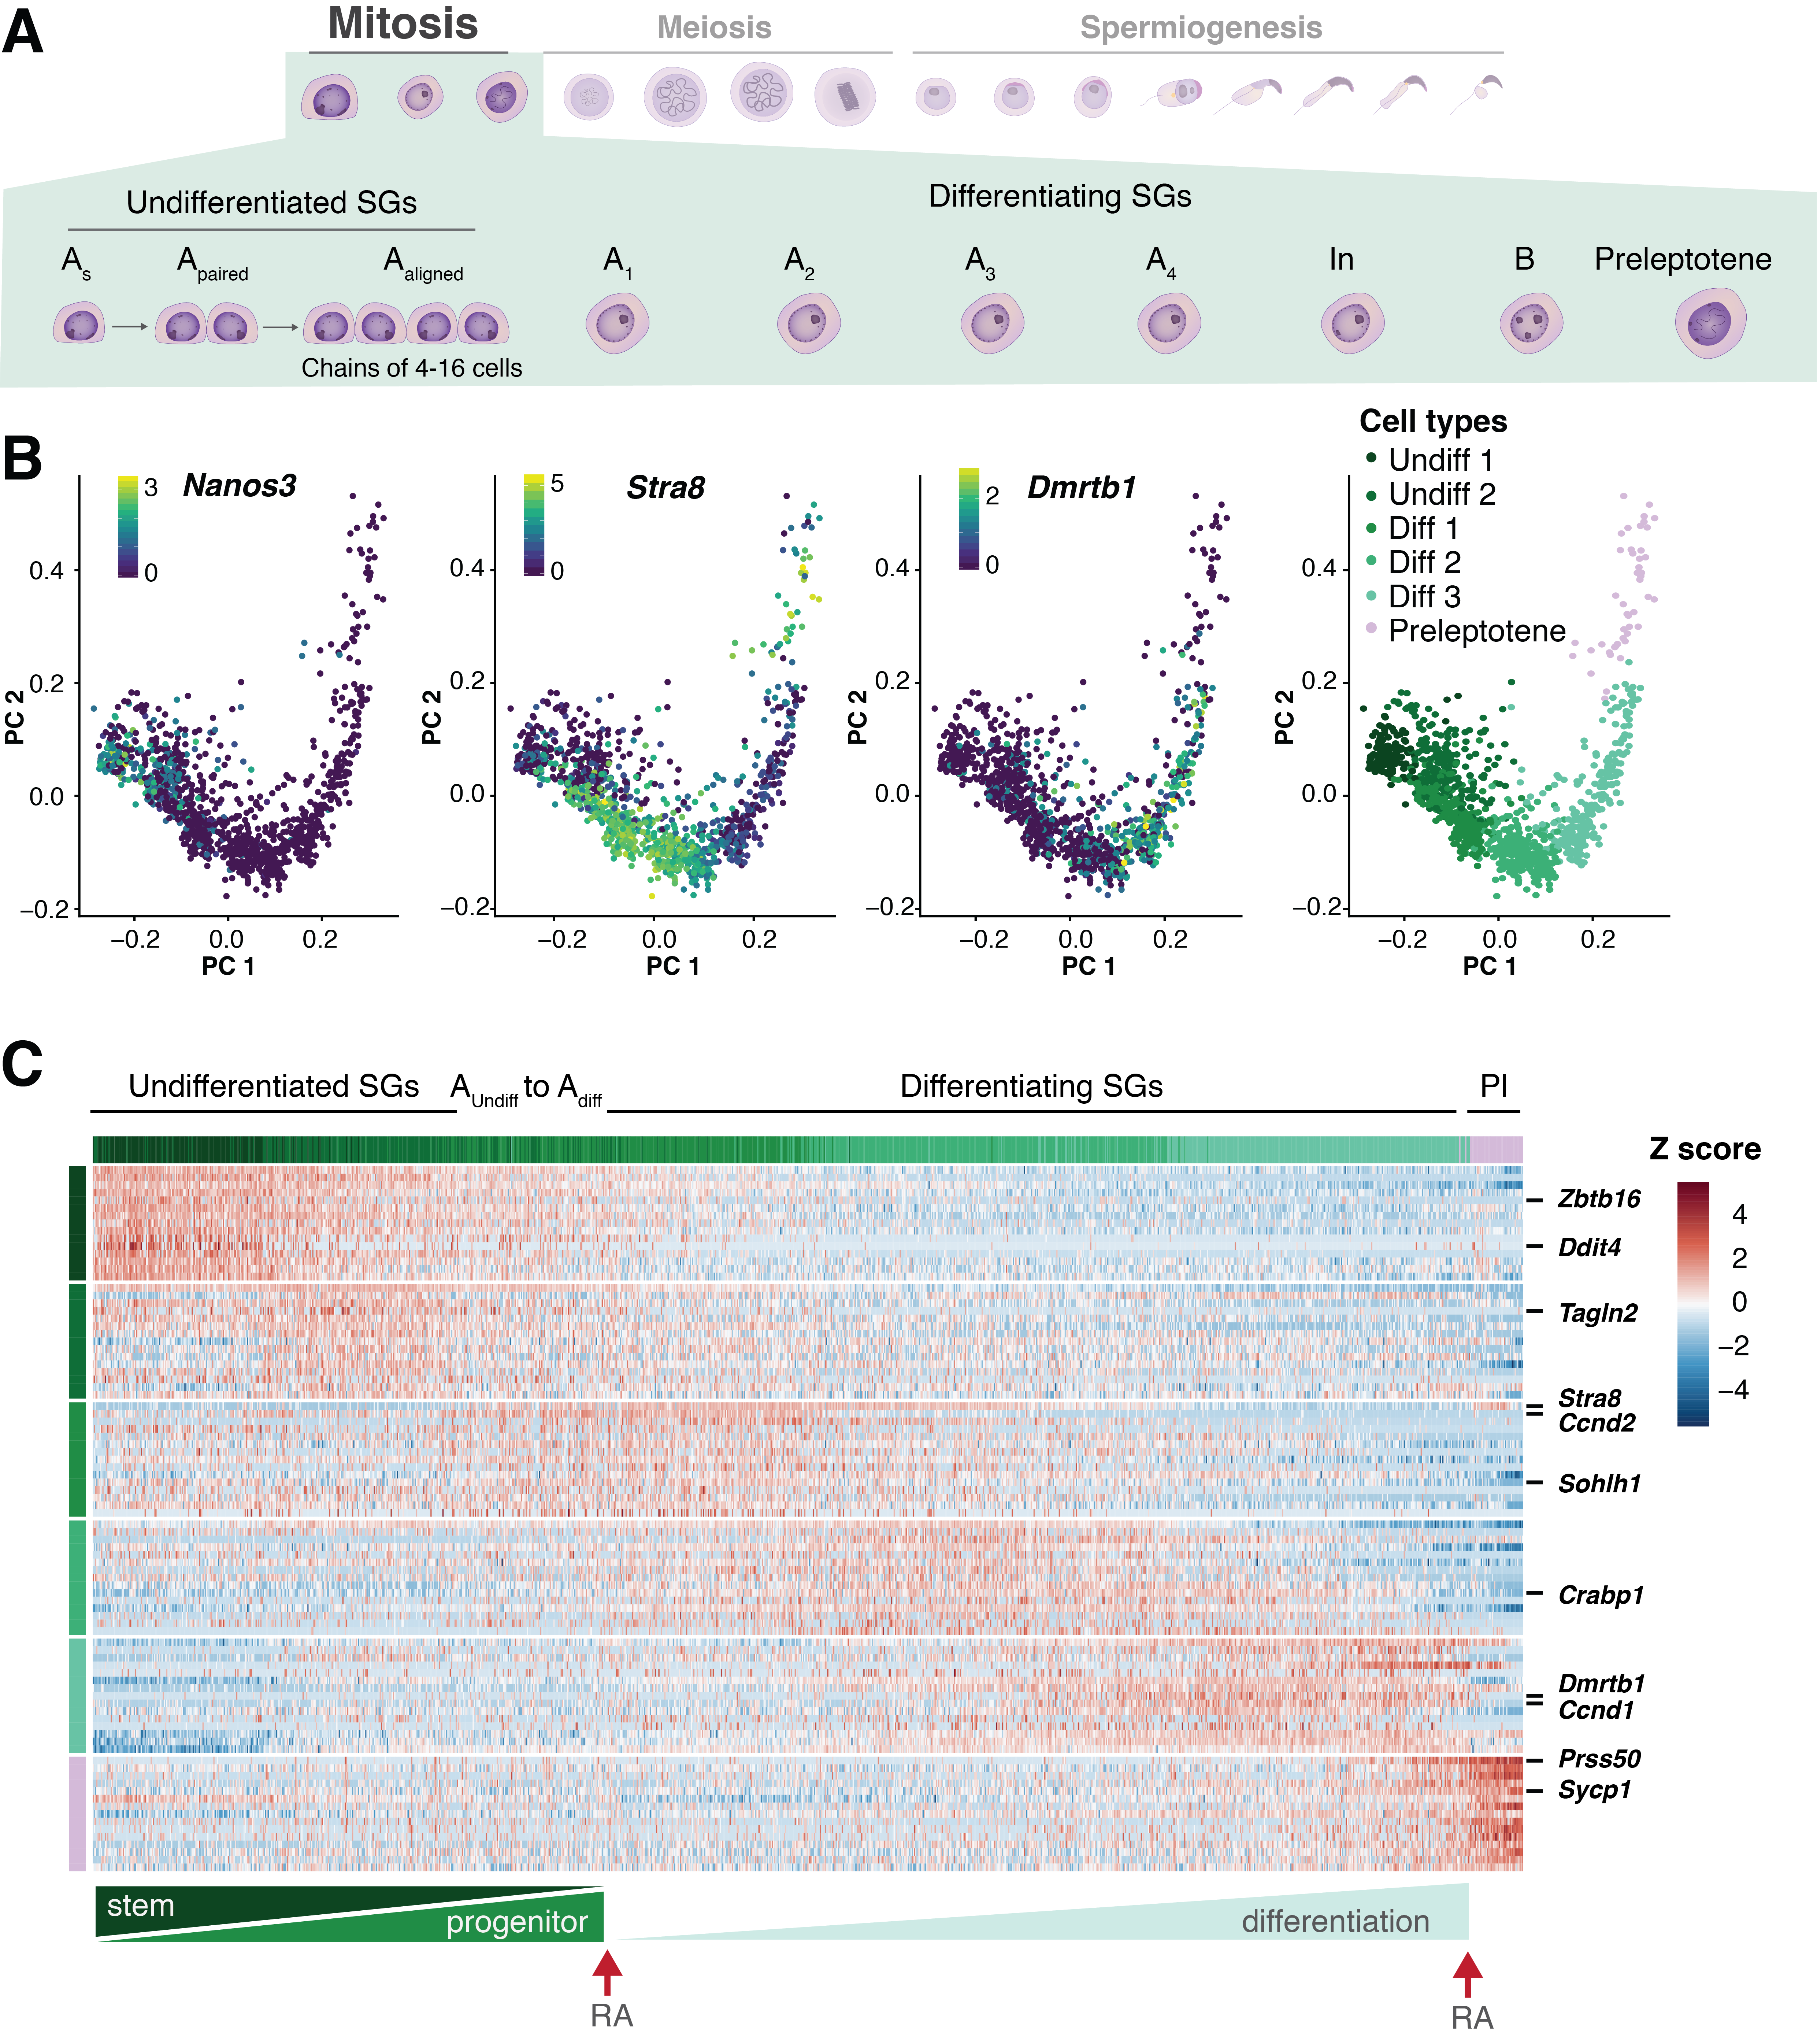
\includegraphics[width=\textwidth]{Fig_6.png}
\caption[Regulatory features that modulate expression noise]{\textbf{Regulatory features that modulate expression noise.}\\
Promoter sequence, number of transcription factor (TF) binding sites (TFBS), number of transcriptional start sites (TSS), enhancer elements, RNA polymerase II (RNAPII) loading, DNA methylation, nucleosome positioning, histone modifications, polycomb repressive complex binding, \glspl{miRNA}, nuclear export of mRNA, ribosome binding and blockage via stem loop formation are features that induce gene-specific intrinsic noise.}
\label{fig0:overview_intrinsic}
\end{figure}

\subsubsection{DNA features}

One of the key regulatory steps prior to RNA synthesis is the binding of \glspl{TF} to specific DNA sequences within the regulatory region (promoter) of a gene which then triggers the controlled production of primary RNA transcripts from the DNA of this gene \citep{Latchman1993}. Mutations in the DNA sequence such as \glspl{SNV} can alter the binding affinity of TFs and therefore the rate at which a gene is expressed \textbf{(Fig.~\ref{fig0:DNA_features})}. A systematic study of the \textit{\gls{TDH3}} gene expression in yeast found that mutations in known \glspl{TFBS} decrease mean expression and increase expression noise. Moreover, Metzger \textit{et al.}, 2015 showed that evolutionary selection removes mutations that increase expression noise and that SNVs with large effects on expression noise show the lowest frequency within sampled yeast strains \citep{Metzger2015}. \\

One of the most widely studied DNA motifs in relation to transcriptional noise is the TATA-box motif in promoters. Generally, TATA-box containing promoters show high levels of transcriptional noise \textbf{(Fig.~\ref{fig0:DNA_features})} \citep{Faure2017} possibly due to a simple activation cycle containing one or few inactive states \citep{Zoller2015}. Stress response genes are enriched for the TATA-box motif and allow an early adjustment to changing environmental conditions \citep{Lopez-Maury2009}. Moreover, TATA-box containing genes show an increased interspecies variability \citep{Tirosh2006} and higher spontaneous mutational variation \citep{Landry2007} indicating an increased evolvability of these particular genes. In an early study, Raser \textit{et al.}, 2004 studied the noisy expression controlled by the budding yeast \textit{\gls{PHO5}} promoter. This promoter contains the TATA-box motif and it has been shown that transcriptional noise is reduced when a mutational modification decreases the TATA-box strength \citep{Raser2004}. A more recent study confirmed this result and found mutations in yeast promoters that eliminate the TATA-box motif which resulted in reduced noise levels for these genes \citep{Hornung2012}. \\

A possible confounding factor for the increased noise of TATA-box containing promoters is the number of TFBSs. Tirosh \textit{et al.}, 2006 detected a two-fold enrichment of TBFSs in TATA-box containing promoters \citep{Tirosh2006}. A later study showed that transcriptional noise scales with increased numbers of TFBSs \textbf{(Fig.~\ref{fig0:DNA_features})} \citep{Sharon2014}. Furthermore, TATA-box containing genes lack enhancing histone marks and their increased variability in expression can therefore be explained by repressed chromatin \citep{Choi2008} (see \textbf{Section \ref{sec0:epigenetic}}).  

\newpage

\begin{figure}[!h]
\centering
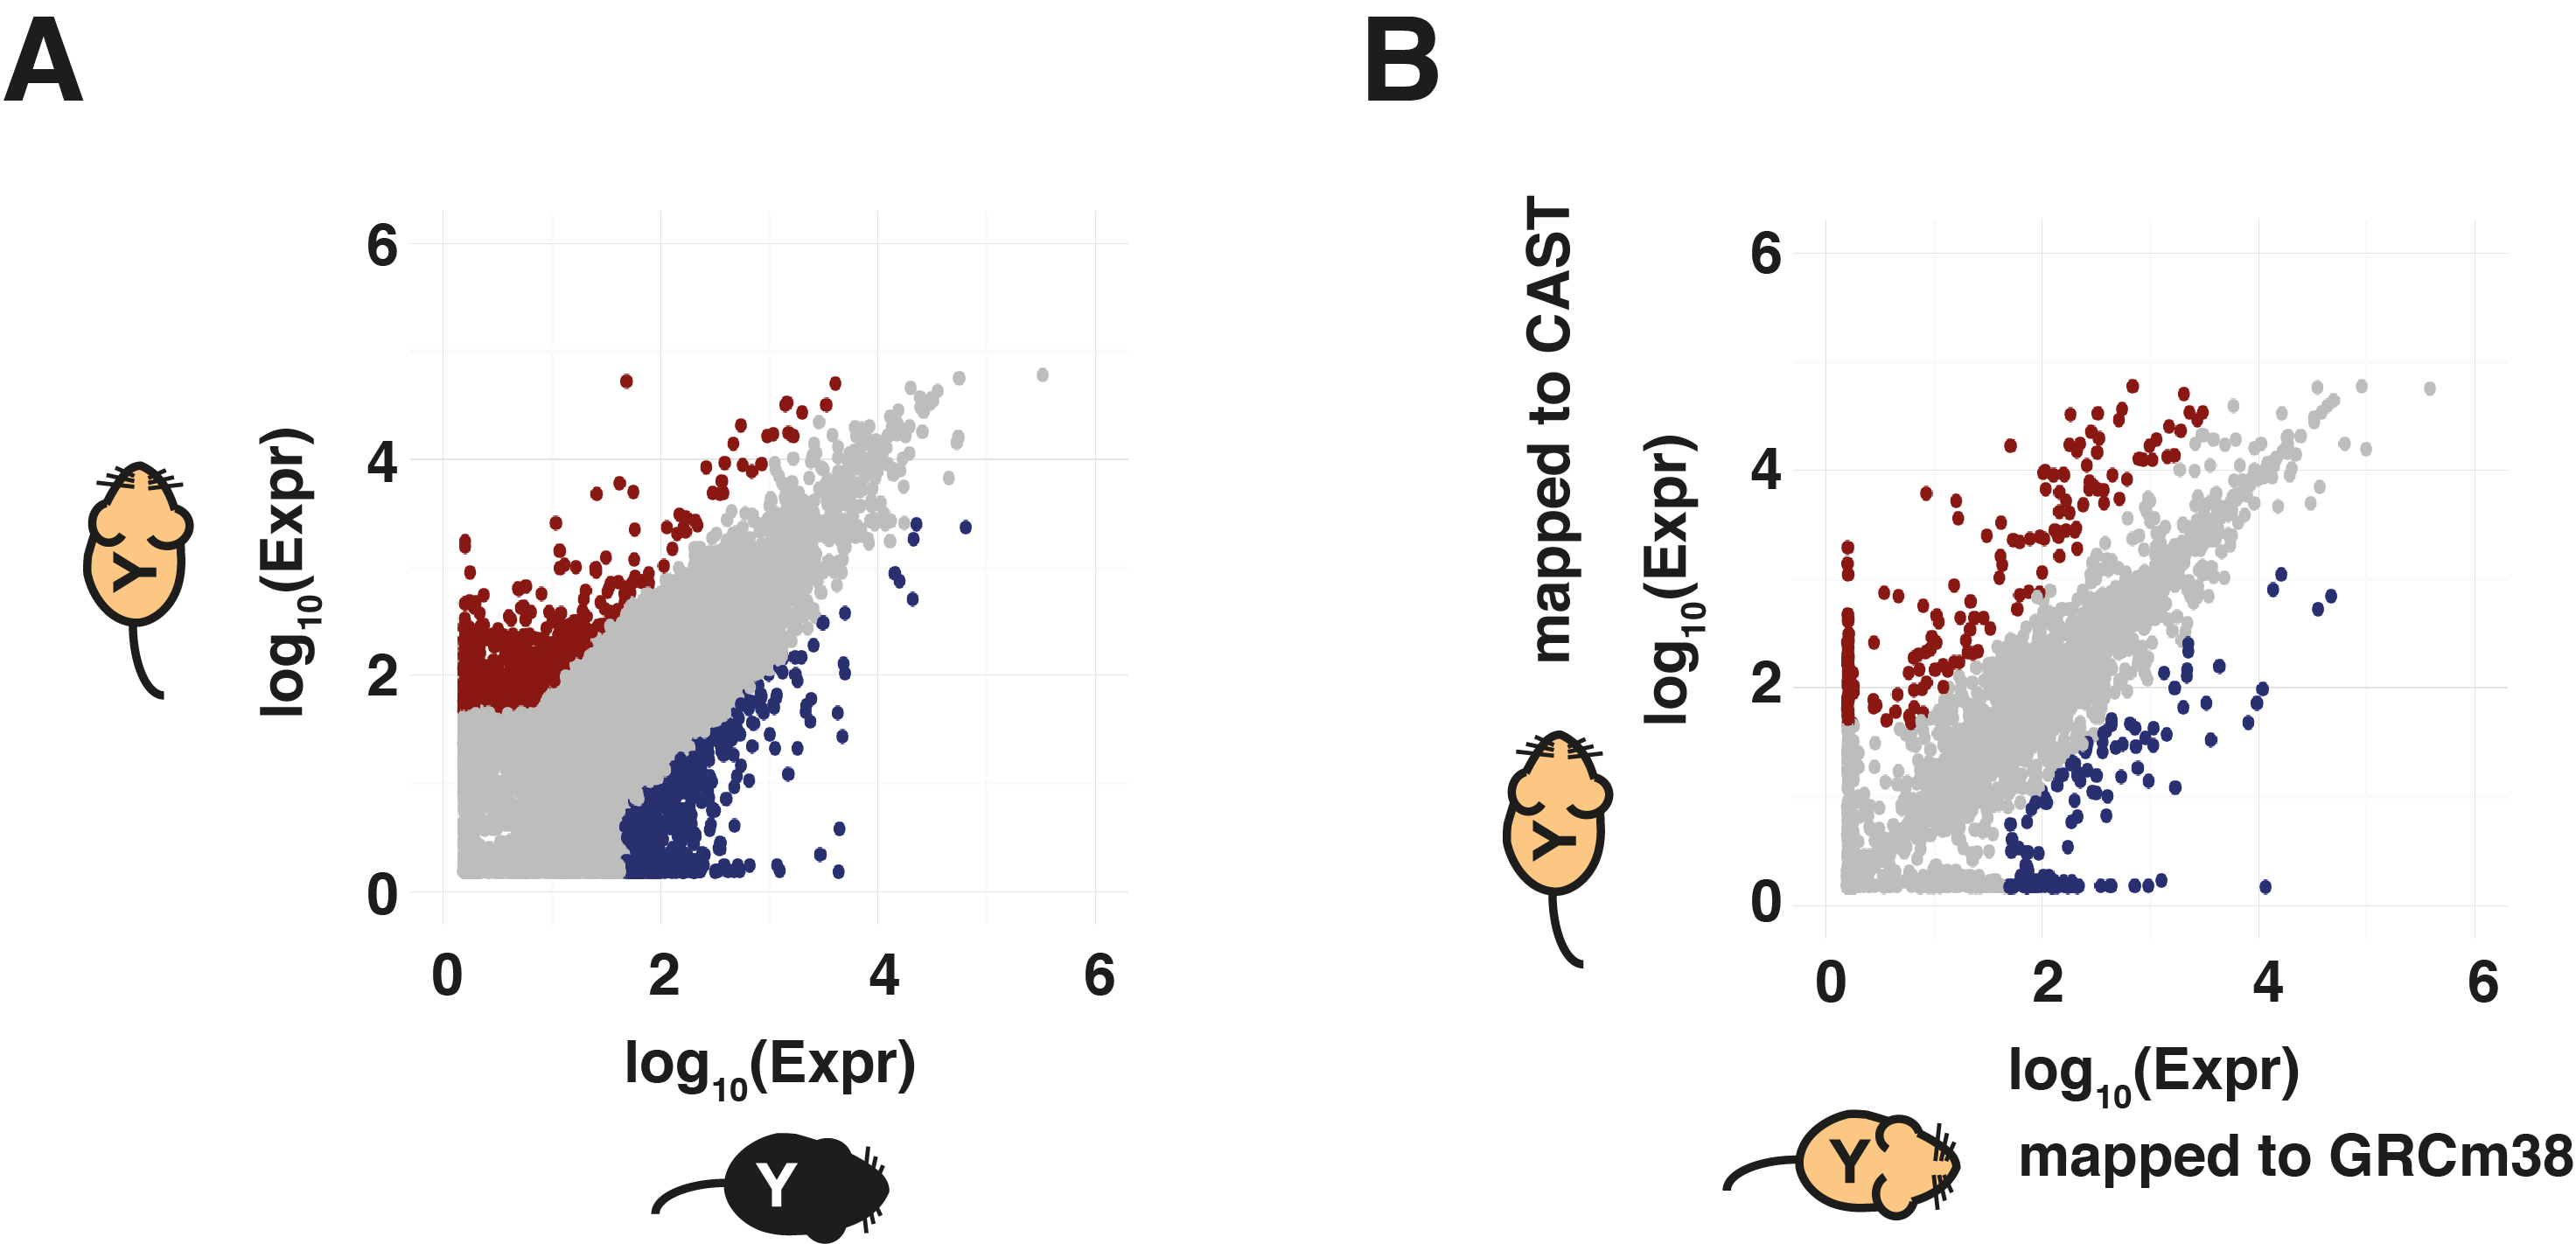
\includegraphics[width=\textwidth]{Fig_7.png}
\caption[Features of the DNA sequence induce expression noise]{\textbf{Features of the DNA sequence induce expression noise.}\\
Mutations of the transcription factor (TF) binding site (TFBS), the presence of a TATA box, increase number of TFBSs, reduced number of transcriptional start sites (TSSs) and reduced copy number of genes can induce transcriptional noise.}
\label{fig0:DNA_features}
\end{figure}

Promoters can be classified based on their shape as narrow with few \glspl{TSS} that predominantly control tissue-specific gene expression and broad promoters with larger numbers of TSSs that control the expression of house keeping genes. Mutations that alter the shape of promoters increase transcriptional noise \citep{Schor2017a}. Furthermore, promoters with one or few TSS show higher levels of expression variability \textbf{(Fig.~\ref{fig0:DNA_features})} \citep{Faure2017}.\\

In addition to SNVs, \glspl{CNV} (usually defined as copy number variability of regions $\geq$ 1kb in comparison to a reference genome) in parts of the genome influence gene expression and contribute to, for example, schizophrenia and autism \citep{Gamazon2015}. Combined analysis of DNA and RNA has shown that genes with low copy number tend to be noisier expressed compared to genes encoded by multiple copies \textbf{(Fig.~\ref{fig0:DNA_features})} \citep{Dey2015}. In the context of monoallelic expression, genes located on the X chromosome show increased mRNA half-life which in turn increases transcript stability and reduces noise to levels of autosomal genes \citep{Faure2017}.

\subsubsection{Epigenetic factors}
\label{sec0:epigenetic}

Epigenetic research is defined as "the study of changes in gene function that are mitotically and/or meiotically heritable and that do not entail a change in DNA sequence" \citep{Wu2001}. Epigenetic factors are generally described as DNA methylation at \gls{CpG} dinucleotides, histone modifications and nucleosome positioning  \citep{Portela2010}. \textbf{Table \ref{tab0:epigenetic}} summarises the relationship between epigenetic features and noisy gene expression. \\

CpG islands are genomic sites of more than 200 bases with a GC content of more than 50\% where DNA methylation can preferentially occur. Methylation of CpG islands in promoters represses transcription while methylation in gene bodies facilitates transcription \citep{Portela2010}.  Recently, the presence of CpG islands in gene bodies but also at the TSS and in promoter regions was linked to a reduction in transcriptional noise \citep{Faure2017}. Similarly, previous findings showed that expression noise scales negatively with gene body methylation \cite{Huh2013}. Morgan and Marioni, 2018 studied the effect of CpG island size on transcriptional noise using scRNA-Seq data. Genes associated with short CpG island promoters tend to be noisier expressed than genes with long CpG island promoters. Furthermore, early response genes during \gls{LPS} stimulation of bone-marrow derived dendritic cells and heregulin stimulation of human breast cancer cells are enriched for those with short CpG island promoters \citep{Morgan2018}. \\

Modifications of histones induce the activation or repression of chromatin and  therefore indirectly modulate gene expression \citep{Suganuma2011}. In an extensive study to link histone modifications to transcriptional noise, Faure \textit{et al.}, 2017 detected several histone modifications in promoter/core promoter motifs, at the TSS and in gene bodies to increase or decrease noise. The repressive \gls{H3K27me3} mark is linked to higher noise levels when present at the TSS, in promoters and in gene bodies. The enhancer related \gls{H3K4me1} mark only increases noise when present at the TSS and in the core promoter sequence while the repressive \gls{H3K9me3} mark increases noise when present in the promoter motif. The activating marks \gls{H3K4me3}, \gls{H3K9ac} and \gls{H3K36me3} are linked to low levels of noise when present in gene bodies. In addition to these single features, bivalent promoters that carry the repressive \gls{H3K27me3} and enhancing \gls{H3K4me3} marks show high levels of transcriptional noise \citep{Faure2017}.\\ 

Polycomp repressive complexes (PRCs) are epigenetic modifiers of histones to repress transcription of developmental genes \citep{Chittock2017}. They can bind together with active \gls{RNAPII} to bivalent promoters and switching between the repressed and active states introduces gene expression variability across a population of cells \cite{Kar2017}. Additionally, deletions of different histone deacetylation complexes (Set3C and Rpd3(L)), that both repress transcription by removing H3K9ac, showed different effects on transcriptional bursting \citep{Weinberger2012}.  Confirming this, a later study indicated that gene body and promoter histone modifications independently influence burst size and burst frequency and therefore regulate mean expression and noise in an uncoupled fashion \cite{Wu2017}. \\

Chromatin is the packaged state of DNA within the nucleus and its central element are nucleosomes. Nucleosomes are made up of eight of the four histones (H3, H4, H2A, H2B) around which 147 bases of DNA twist. An array of histone modifying enzymes exits that regulate the opening or closing of the chromatin; termed heterochromatin and euchromatin respectively \citep{Kouzarides2007}. Tirosh \textit{et al.}, 2008 showed that promoters with high nucleosome occupancy close to the TSS tend to display a high range of expression levels across varying conditions (transcriptional plasticity). Distant nucleosome-rich regions are on the other hand associated with low transcriptional noise \citep{Tirosh2008}. Nucleosome covered promoters display shorter transcriptional rates, which in turn explains increased transcriptional noise for these promoters \cite{Dey2015}. Single-cell measures indicate cell-to-cell variations in nucleosome positioning around the \textit{PHO5} promoter upon stress induction. Even in the non-stressed state, a small fraction of cells exhibit nucleosome free regions at the promoter which explains low and possibly noisy expression of \textit{PHO5} \citep{Small2014}. Deletion of chromatin remodeling complexes that remove nucleosomes upon transcription factor binding results in increased transcriptional noise compared to wild-type cells \citep{Raser2004}. 

\newpage

Boundaries between heterochromatin and euchromatin are controlled by boundary elements, such as the transcription factor \Gls{CTCF}, that recruit chromatin modifying factors \citep{Kouzarides2007}. CTCF also regulates transcription by activating or repressing promoters and regulates distant chromatin interactions \citep{Kim2015a}. Recent studies suggest that long-range enhancer-promoter interactions modulate transcriptional noise. Interference of CTCF-mediated enhancer-promoter contact either by CTCF knock-out or CTCF-binding site deletion leads to increased expression variability in selected genes \citep{Ren2017}. Enhancers are cis-regulatory elements of non-coding DNA containing TFBSs, that regulate the expression of neighbouring genes \citep{Blackwood1998}. Genes within super-enhancer loci, a region with multiple enhancers, controlling pluripotency master regulators show high levels of variability in expression and down-stream targets of these master regulators show similar co-variation across mESCs \citep{Faure2017}.

\begin{table}[hb	]
\centering
\caption{Epigenetic control of transcriptional noise}
\label{tab0:epigenetic}
\begin{tabular}{l l c c}
\toprule
\toprule
 & Feature & Noisy & Stable \\ 
\midrule
\midrule
\multirow{3}{*}[-2pt]{DNA methylation} & CpG islands &  & \checkmark{} \\
\cmidrule{2-4}
& Short CpG islands & \checkmark{} &  \\
\cmidrule{2-4}
& Gene body methylation &  & \checkmark{} \\
\midrule
\multirow{7}{*}[-2pt]{Histone modification} & H3K27me3 (TSS, promoter, gene body) & \checkmark{}  & \\
\cmidrule{2-4}
& H3K4me1 (TSS, promoter) & \checkmark{}  & \\
\cmidrule{2-4}
& H3K9me3 (promoter) & \checkmark{}  & \\
\cmidrule{2-4}
& H3K4me3 (gene bodies) &  & \checkmark{}\\
\cmidrule{2-4}
& H3K9ac (gene bodies) &  & \checkmark{} \\
\cmidrule{2-4}
& H3K36me3 (gene bodies) &  & \checkmark{} \\
\cmidrule{2-4}
& H3K27me3 and H3K4me3 & \checkmark{}  & \\
\midrule
\multirow{3}{*}[-2pt]{Nucleosome position} & Nucleosome rich promoters & \checkmark{} & \\
\cmidrule{2-4}
& Distant nucleosome rich regions &  & \checkmark{} \\
\cmidrule{2-4}
& Deletion of nucleosome remodelling complexes & \checkmark{}  & \\
\midrule
\multirow{7}{*}[-2pt]{Genome architecture} & CTCF knock-out & \checkmark{} & \\
\cmidrule{2-4}
& CTCF binding site depletion & \checkmark{} & \\
\cmidrule{2-4}
& Clustered genes &  & \checkmark{} \\
\cmidrule{2-4}
& Nuclear-lamina associated genes & \checkmark{} & \\
\bottomrule
\bottomrule
\end{tabular}
\end{table} 

\newpage

Moreover, the positioning of genes on the genome controls expression noise with densely clustered genes being less noisy expressed in comparison to non-clustered genes \citep{Kustatscher2017}. Additionally, genes positioned next to “noisy” genes display higher levels of transcriptional variability compared to genes that are located in proximity to “stable” genes \citep{Kar2017}. Expression noise is also increased for genes that are located in a repressed neighborhood, namely active genes in constitutive nuclear lamina-associated domains \citep{Faure2017}.

\subsubsection{Transcriptional features}

Transcription is initiated by TFs binding to specific regulatory DNA sequences followed by recruitment of RNAPII, RNA synthesis and RNA degradation. As discussed above, promoter architecture, namely the location and accessibility of TFBS and RNAPII binding sites, dictates mean expression and transcriptional noise. \\

In bacteria, the intracellular physical distance between TF source and the promoter sequence influences expression variability. TF expression proximal to their target genes results in less noisy expression compared to regulator sources distant to the promoter sequence \citep{Goni-Moreno2017}. Once TFs bind to their target sequence, Carey \emph{et al.}, 2013 showed that mean expression to noise ratio is promoter dependent while in the majority of cases, noise negatively scales with mean expression \citep{Carey2013}. \\

Similar to TF binding dynamics, the assembly of RNAPII complexes modulates transcriptional noise. An early study identified the connection between paused RNAPII and synchronous expression of target genes. Genes without pre-loaded RNAPII show more stochastic activation patterns \citep{Boettiger2009}. This finding has later been confirmed using scRNA-Seq data while increased variability was detected for genes with non-pause RNAPII across the full range of expression levels \textbf{(Fig.~\ref{fig0:RNAPII})} \citep{Day2016}.\\

\begin{figure}[!h]
\centering
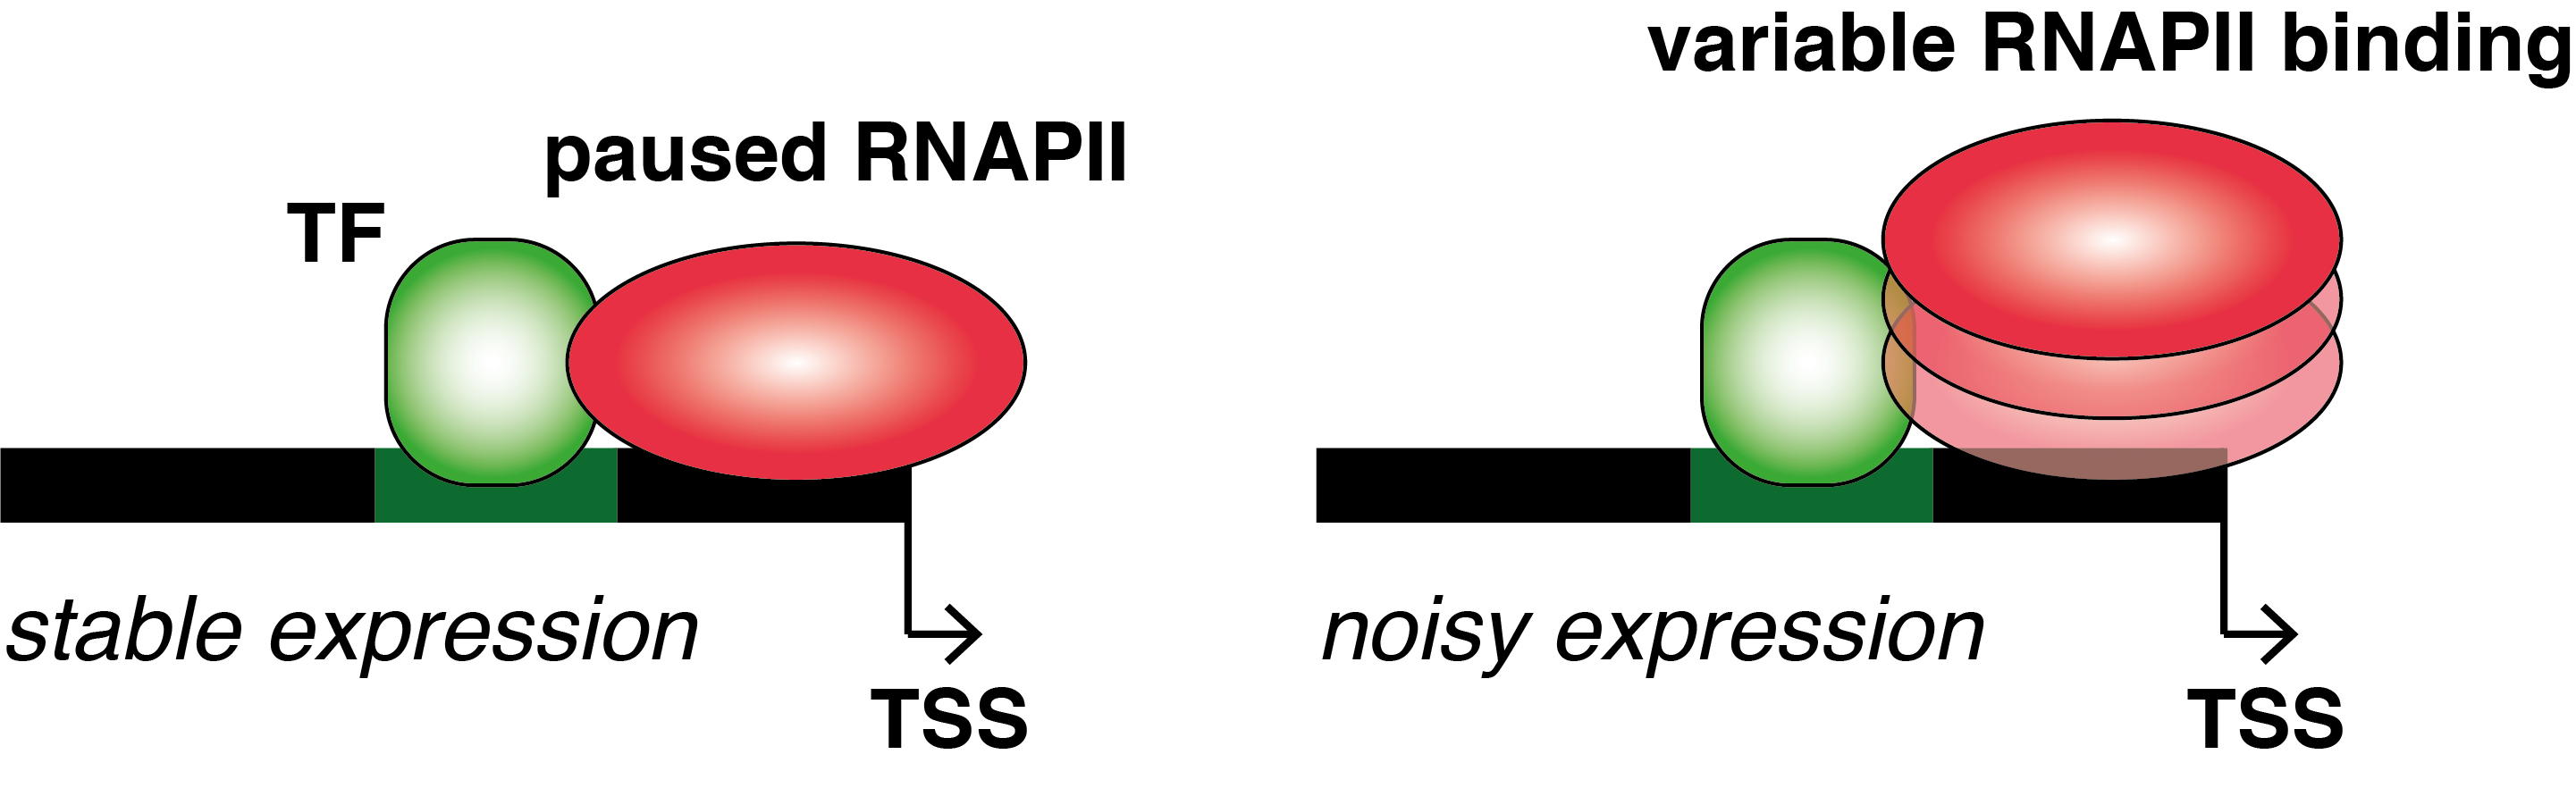
\includegraphics[width=0.7\textwidth]{Fig_8.png}
\caption[RNAPII pausing reduces transcriptional noise]{\textbf{RNAPII pausing reduces transcriptional noise.}\\
Left: Pre-loaded RNA polymerase II (RNAPII) allows direct transcription upon transcription factor (TF) binding. Right: RNAPII recruitment induces gene expression variability.}
\label{fig0:RNAPII}
\end{figure} 

\newpage

\subsubsection{Post-transcriptional and translational features}

After synthesis, pre-RNAs are polyadenylated and spliced to form mRNA that relocates from the nucleus to the cytoplasm where translation occurs to synthesise proteins \cite{Glisovic2008}. On the post-transcriptional and translational level, mRNA localization, structure, degradation and translation have been shown to influence cell-to-cell variations in protein abundance.

Upon transcriptional activation, RNAs are produced in burst-like patterns while burst frequency modulates mean expression and noise, and burst size influences solely mean expression \citep{Hornung2012}. While bursty transcript synthesis introduces stochastic fluctuations in nuclei between cells, active export of mRNAs into the cytoplasm can dampen this source of variability \textbf{(Fig.~\ref{fig0:posttranscriptional})} \citep{Battich2015a}. Reduces cytoplasmatic noise has also been shown for two nuclearly retained genes in the mammalian liver. Furthermore, this mode of noise control was proposed to be active across a range of metabolic tissues \cite{BaharHalpern2015a}.\\

\begin{figure}[!h]
\centering
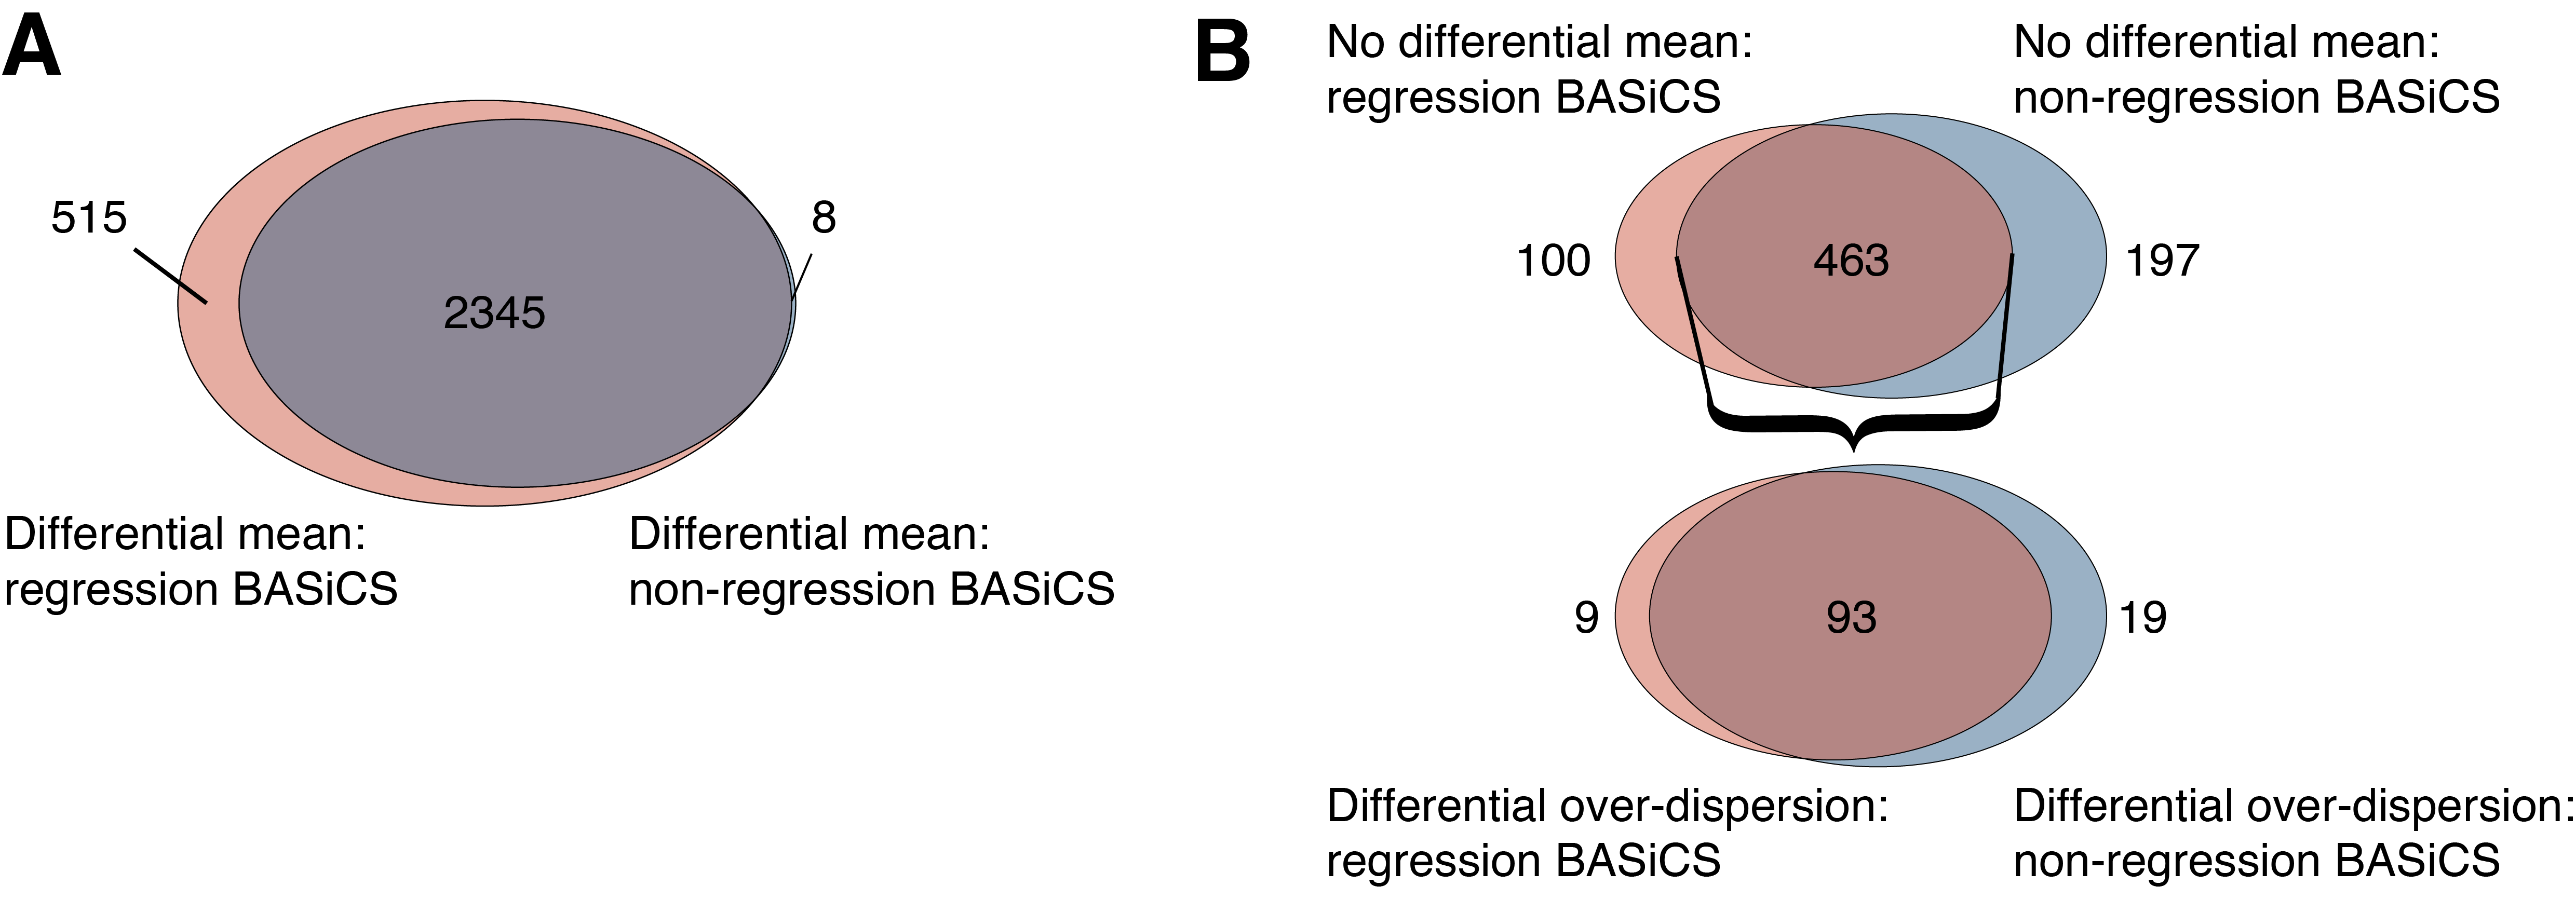
\includegraphics[width=\textwidth]{Fig_9.png}
\caption[Post-transcriptional regulation to control noisy expression]{\textbf{Post-transcriptional regulation to control noisy expression.}\\
Bursty expression introduces nuclear variation in transcript abundance that is buffered due to retention at the nuclear membrane. Within the cytoplasm, micro RNAs degrade lowly expressed genes to reduce expression noise. Deletion of the ribsosome binding site as well as stem loop formation increase variability in protein abundance across cells. Arrows indicate either increased (red) or decreased noise (green) dependent on the regulatory mechanism.}
\label{fig0:posttranscriptional}
\end{figure} 

\newpage

Within the cytoplasm, mRNAs are subject to translation or degradation. At this stage, stochasticity from bursty gene expression is propagated to variation in protein abundance. The availability of mRNAs for translation is not only dictated by their syntheses but also their degradation rate. mRNA degradation is accelerated by recognition of micro RNAs. This process has been shown to preferentially reduce noise levels for lowly expressed genes in mESCs to possibly retain cellular identity \textbf{(Fig.~\ref{fig0:posttranscriptional})} \citep{Schmiedel2015}. Similarly, temporal averaging of long-lived transcripts reduces noise in mRNA abundance. In that way, increased transcript stability compensates for noise introduced by the single-allele expression of genes on chromosome X \citep{Faure2017}.  \\

In addition to noise introduced by stochastic processes on the transcriptional level, the recognition and binding of ribosomes to mRNAs for translation initiation features a source for variations in protein abundance. Modulating translational efficiency by mutating the ribosome binding site and initiation codon showed an interaction between translation and variation in protein abundance \textbf{(Fig.~\ref{fig0:posttranscriptional})} \citep{Ozbudak2002}. Additionally, mRNA secondary structure formed by stem loops and ploy(G) motifs affects translation initiation and increases noise in protein levels \textbf{(Fig.~\ref{fig0:posttranscriptional})} \citep{Dacheux2017a}.

\subsection{Extrinsic noise}

Extrinsic noise within a cell population arises from cells being in different regulatory states. Here, differences in cellular components introduce variation in mRNA and protein abundance. Examples for cell states in otherwise homogeneous populations are characterized by differences in metabolism, cell cycle, volume, cell-to-cell and environmental signalling as well as cell density. It has been shown that extrinsic noise forms a major contribution to variations in gene expression and that transcript distributions can be predicted from the cellular state, population context and microenvironment \citep{Battich2015a}.

\subsubsection{Cell cycle}

Cell cycle has been widely discussed to form a crucial source of extrinsic noise \citep{Colman-Lerner2005a, Newman2006}). In yeast populations, differences in transcriptional activities between the G1 and S/G2/M phases of the cell cycle lead to large-scale transcriptional heterogeneity across cell populations \textbf{(Fig.~\ref{fig0:extrinsic})} \citep{Zopf2013}. Under nutrient-poor conditions, growth rate is reduced and noise is elevated due to cells being in different cell-cycle stages \citep{Keren2015}.  Even under optimal growth conditions for mESCs (2i media), cell cycle related genes show strong heterogeneity in expression across the cell population \citep{Kolodziejczyk2015cell}. Nonetheless, sorting cells into similar cell cycle stages did not drastically reduce noise levels \citep{Raser2004}. When quantifying cell-to-cell variation, cell cycle induced extrinsic noise is often seen as unwanted variation and can mask more subtle transcriptional heterogeneity. Computational methods have been developed to correct for this confounding effect to enhance the underlying noise signal \citep{Buettner2015, Buettner2017}. 

\begin{figure}[!h]
\centering
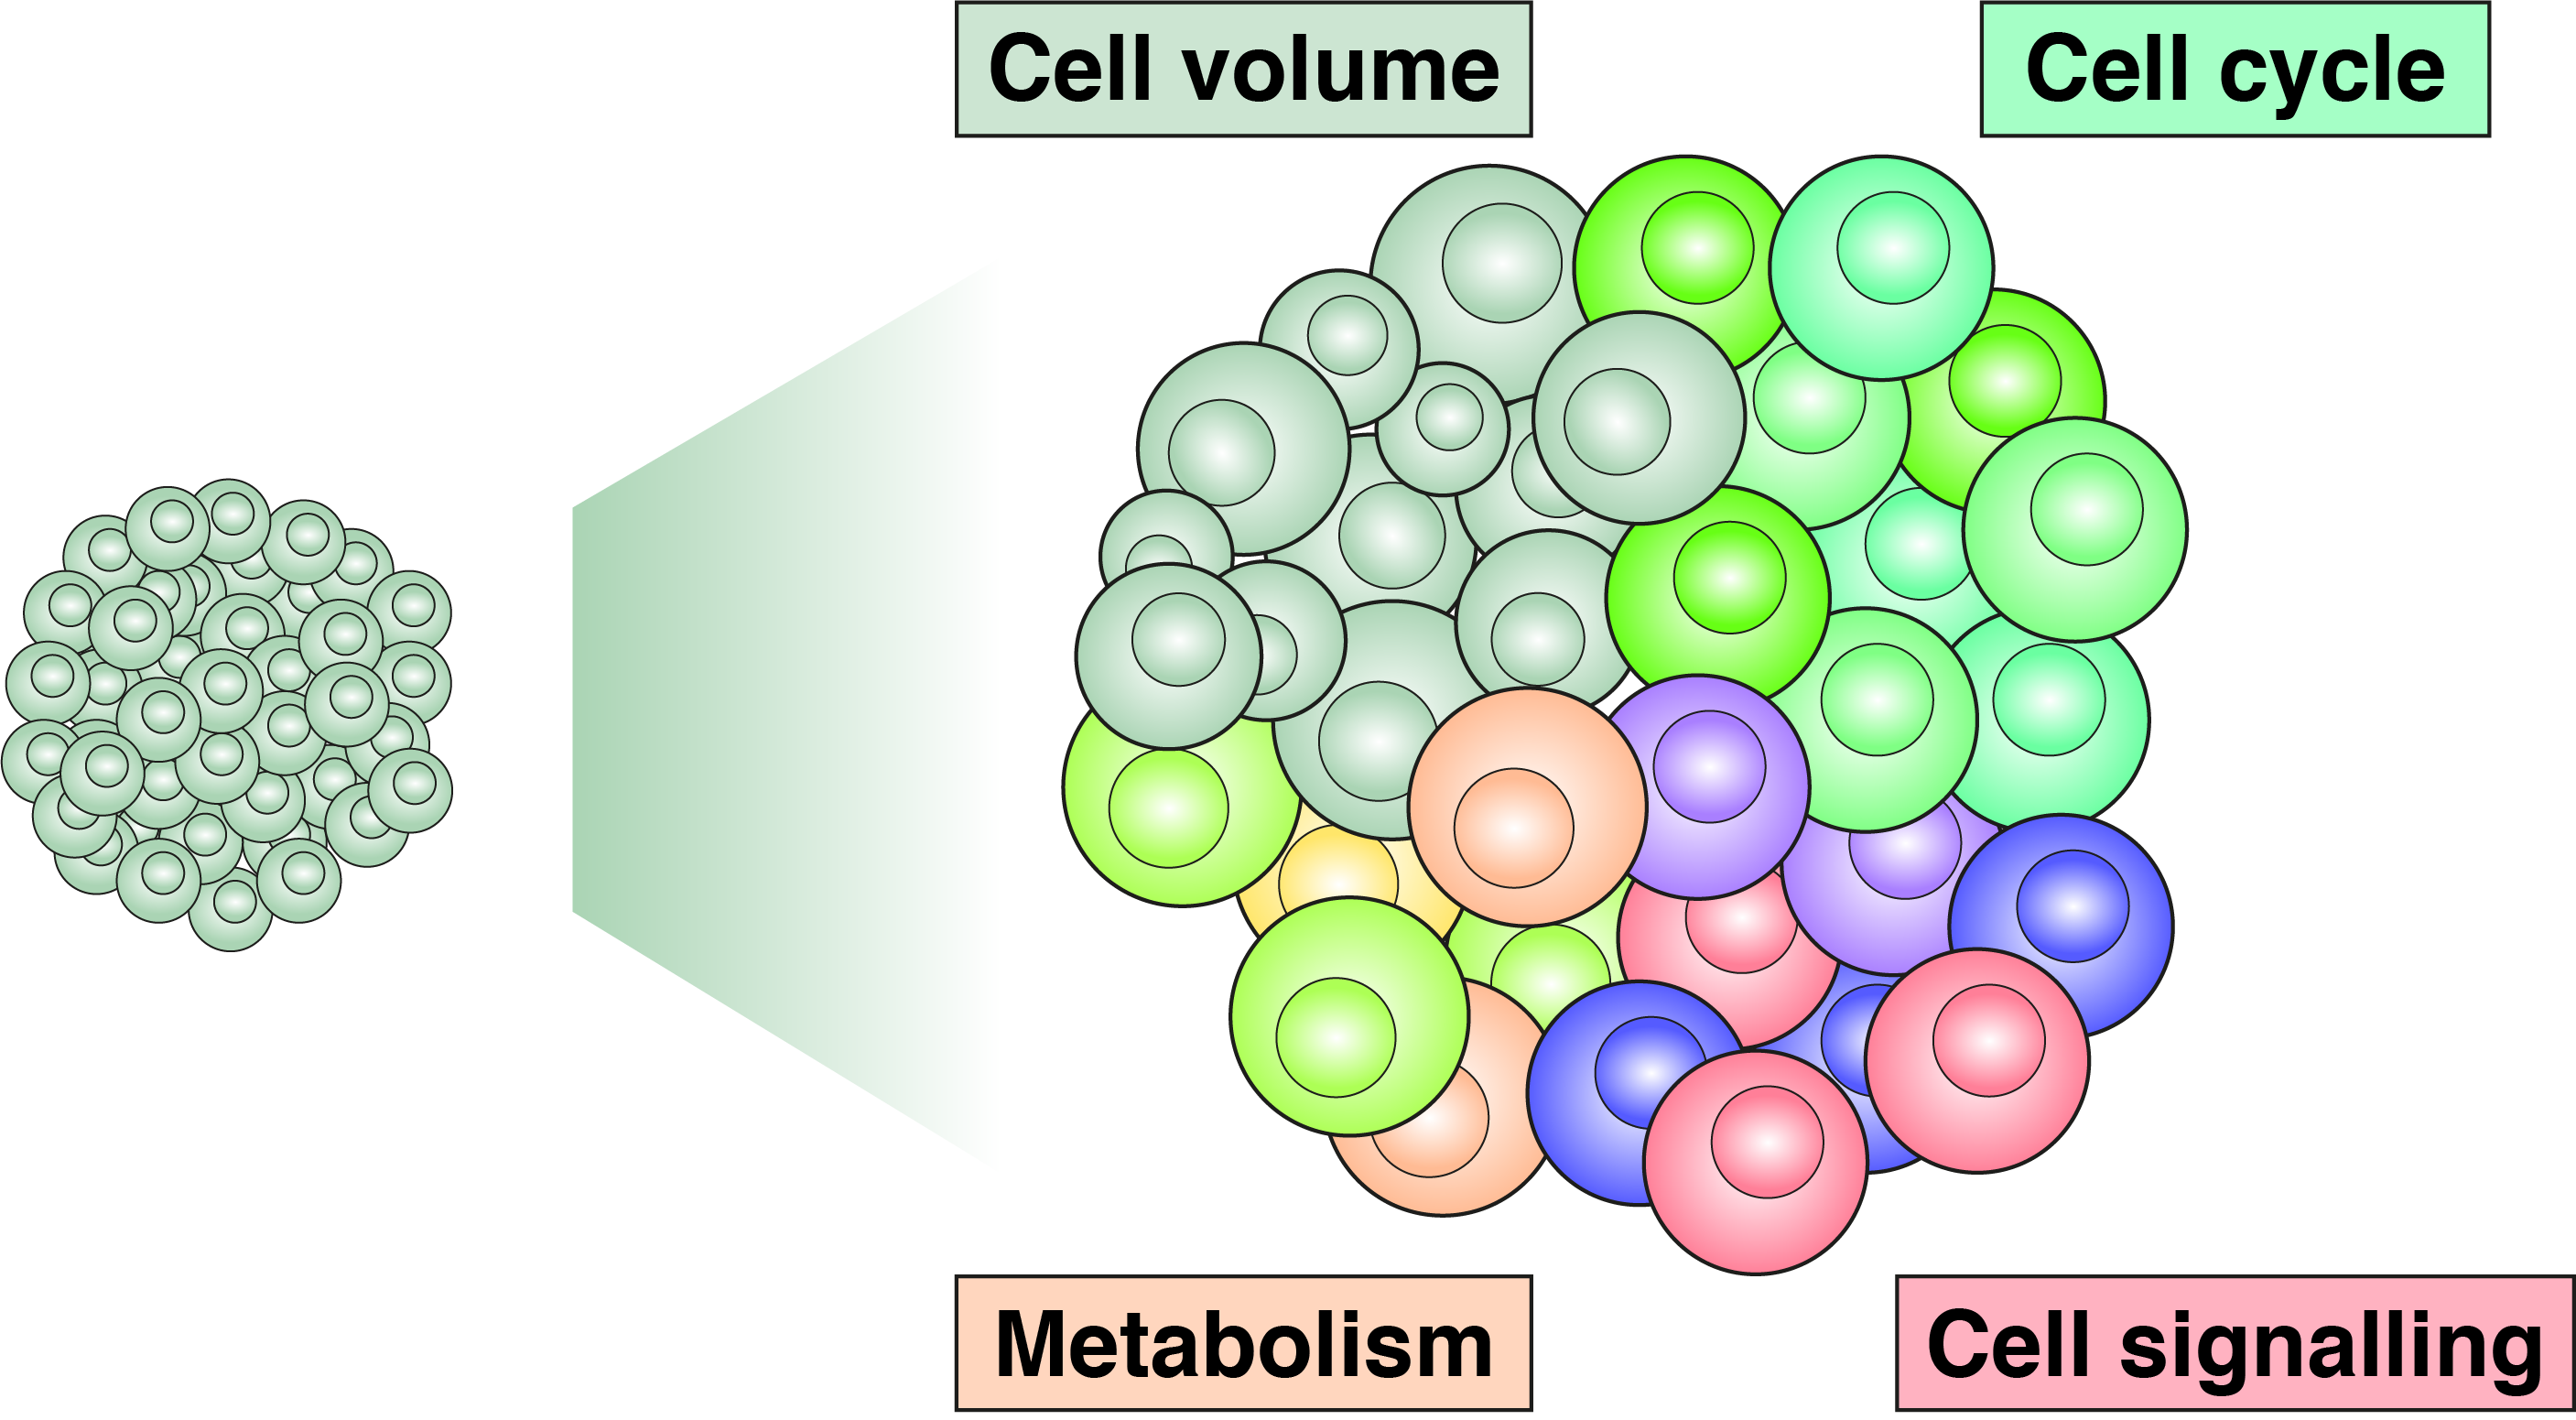
\includegraphics[width=0.7\textwidth]{Fig_10.png}
\caption[Differences in cell states induce extrinsic noise]{\textbf{Differences in cell states induce extrinsic noise.}\\
Within a homogeneous population of cells (left), individual cells reside in different cellular states (e.g.~cell cycle, cell signalling, metabolism) and show differences in cellular volume.}
\label{fig0:extrinsic}
\end{figure} 

\subsubsection{Cell volume}

Cellular volume provides another explanation for global differences in mRNA content between individual cells introducing large-scale transcriptional heterogeneity \textbf{(Fig.~\ref{fig0:extrinsic})}. Even though cell volume changes during cell cycle progression, within each phase cell volume varied as much as across all phases. It has been shown that mRNA counts scale with cellular volume to maintain transcript concentrations within each cell \citep{Kempe2015, Padovan-Merhar2015, Zhurinsky2010}. To avoid this source of heterogeneity, normalization approaches correct for differences in mRNA content between individual cells \citep{Vallejos2017}.

\subsubsection{Metabolism}

The effect of metabolic fluctuations has been studied in \textit{E. coli} populations. Variations in biochemical reactions are induced by noise in the expression of their corresponding catalytic enzymes. Changes in metabolism are then coupled to varying growth rates of individual cells, which in turn introduces large-scale transcriptional heterogeneity in cell populations \textbf{(Fig.~\ref{fig0:extrinsic})} \citep{Kiviet2014}.  

\subsubsection{Expression capacity}

Fluctuations in the expression capacity of cells due to quantitative differences in RNAPII or ribosomes induce global variability among the majority of proteins \citep{Colman-Lerner2005a}.

\subsubsection{Cell signalling}

A different source of extrinsic noise is the intra- or inter-cellular signalling state of individual cells. Fluctuations in membrane bound or cytoplasmic proteins lead to inconsistent transmission of signalling stimuli as exemplified by variability in TRAIL-induced apoptosis \citep{Spencer2009}. Similarly, variations of regulators in the \gls{ERK} signalling pathway introduce downstream variability in nuclear response \textbf{(Fig.~\ref{fig0:extrinsic})}. The degree of which nuclear ERK response is varied depends on the position of the regulator in the topology of the signalling pathway \citep{Iwamoto2016}. In \textit{C. elegans}, perturbation of the Wnt signalling pathway displayed different degrees of variability in expression of the key Hox gene for Q neuroblast migration, \textit{mab-5}. It has been proposed that extrinsic noise, in this case the strength of the Wnt signal, modulates intrinsic variation in the expression of \textit{mab-5} \citep{Ji2013}. 

\subsubsection{Physical constrains}

\begin{wrapfigure}{r}{0.5\textwidth}
\centering    
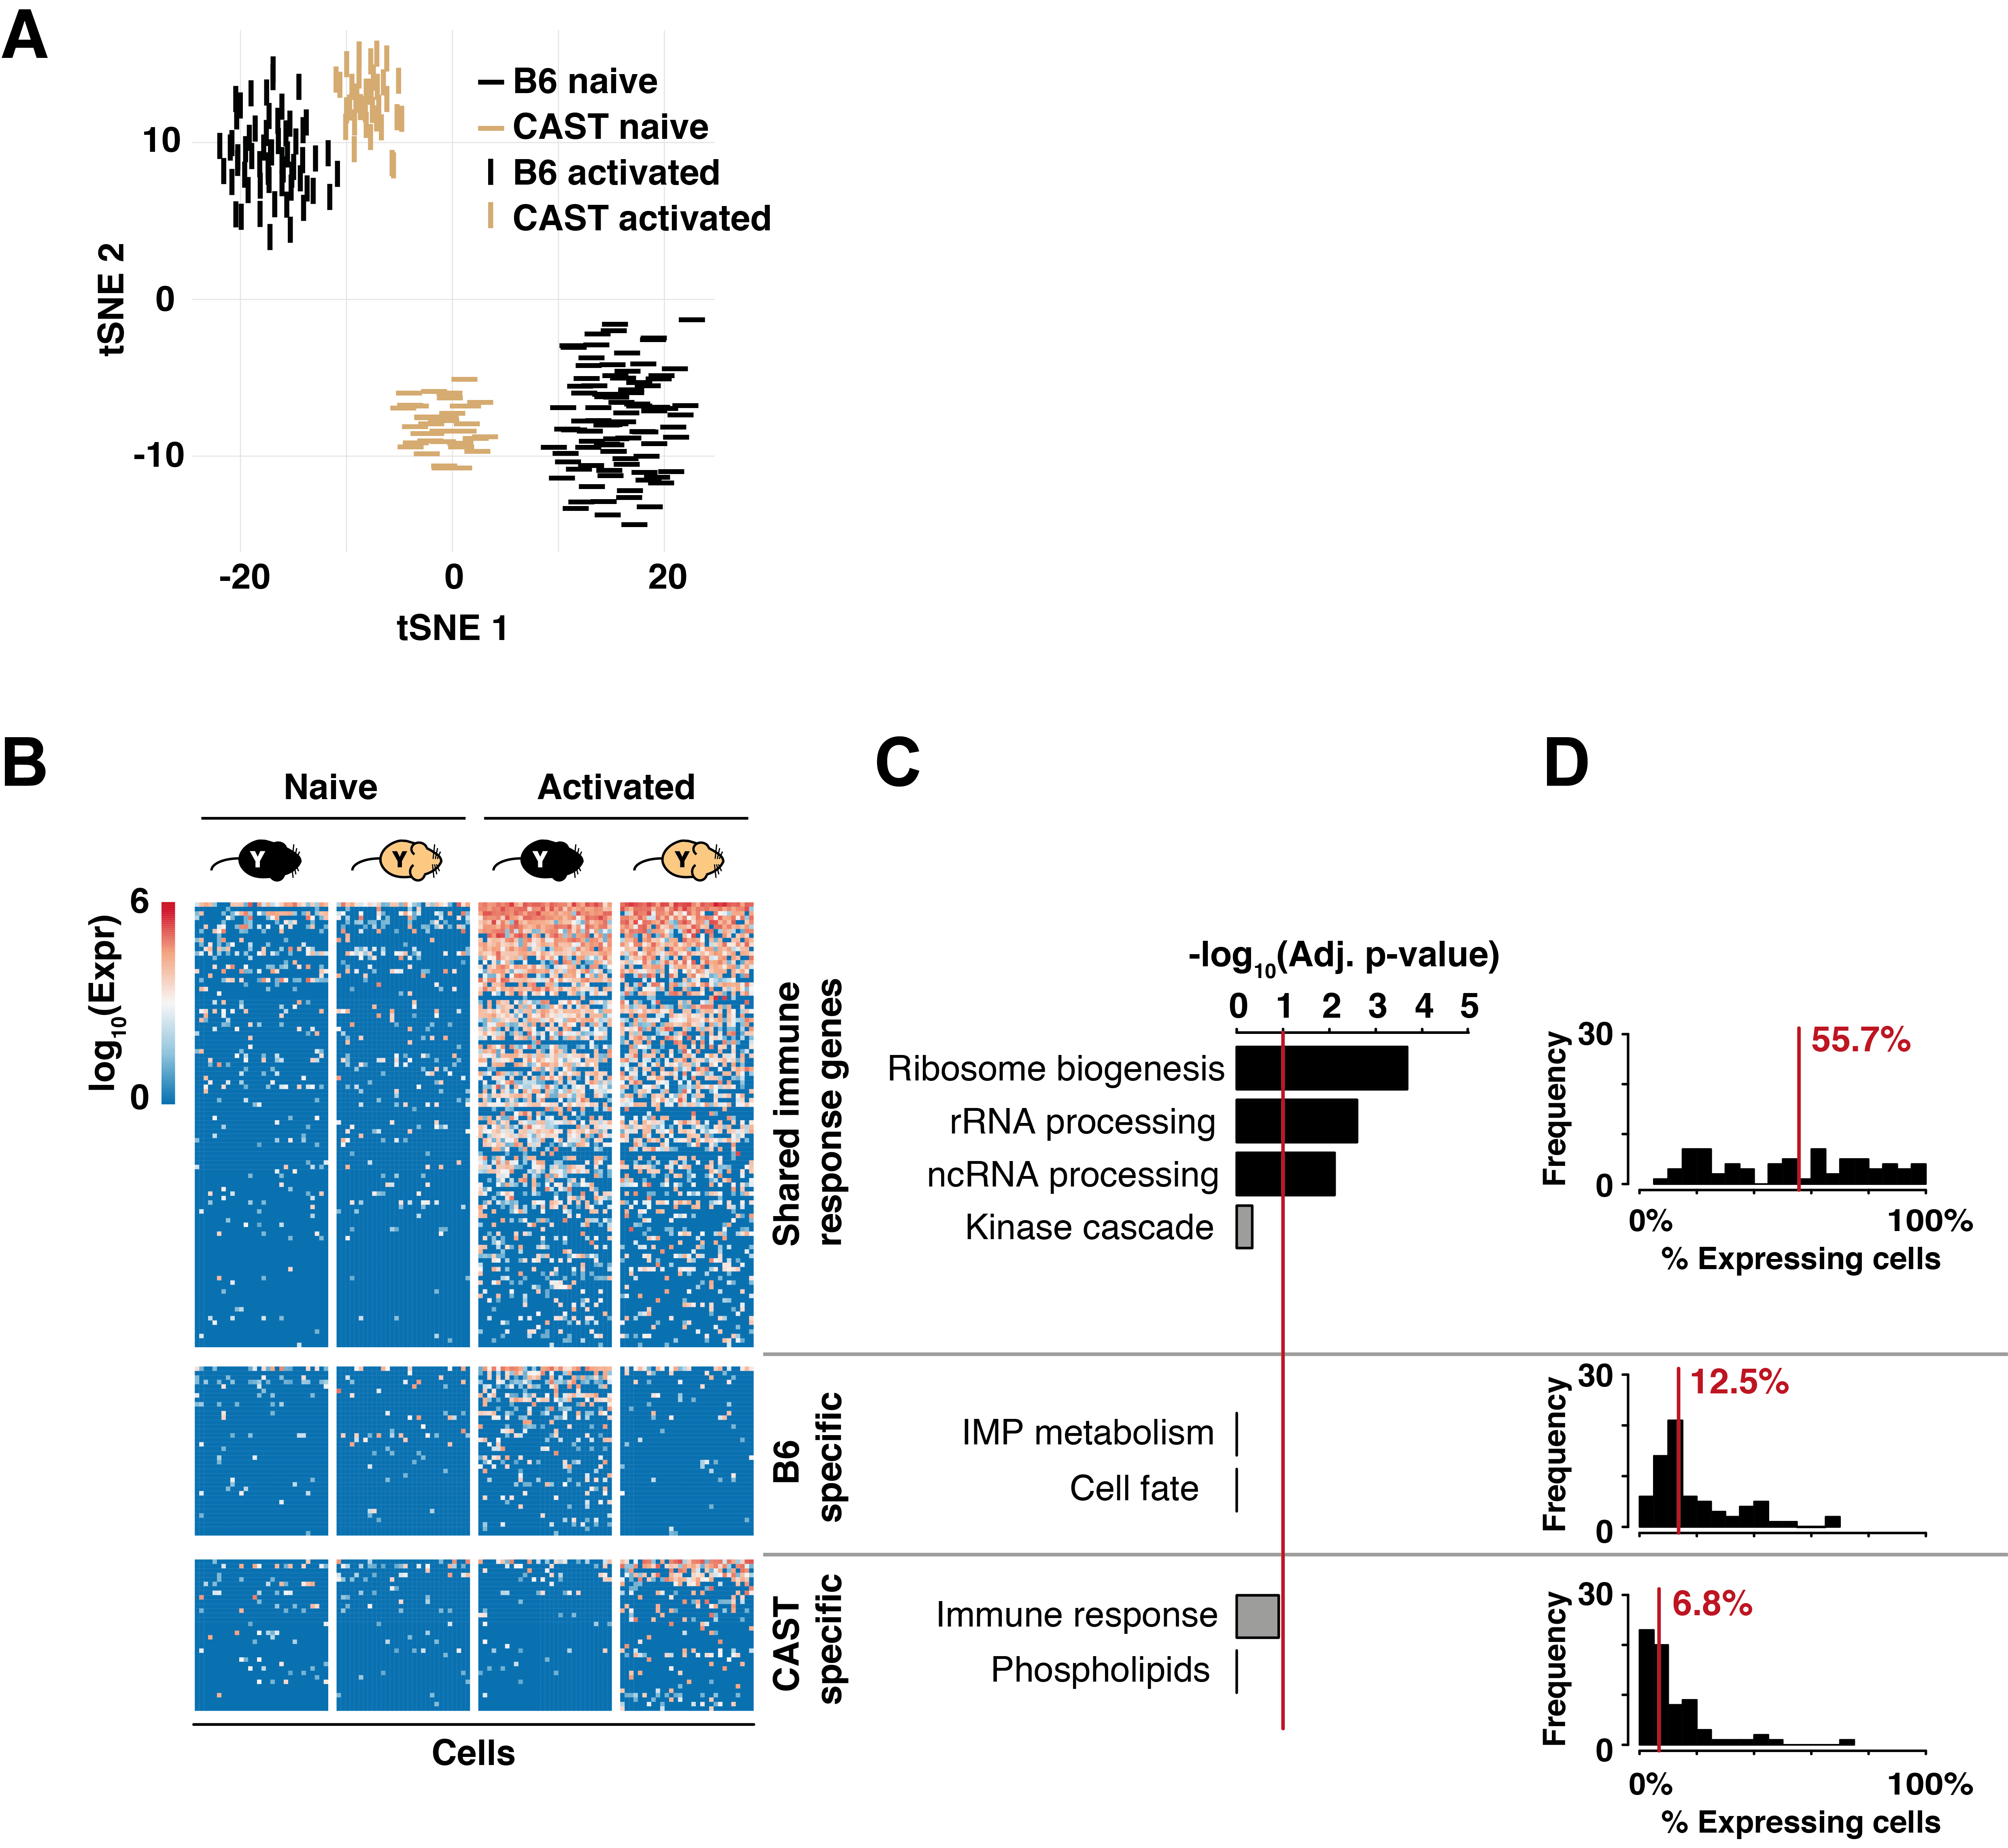
\includegraphics[width=0.48\textwidth]{Fig_11.png}
\caption[Physical constrains induce heterogeneous expression patterns.]{\textbf{Physical constrains induce heterogeneous expression patterns.} \\
Cell density increases during the expansion of a homogeneous population of cell forming patches with high and low density and pushing cells to the edge of the population. Based on these physical constrains, cells change their transcriptional programme inducing variability across the population.}
\label{fig0:constrains}
\end{wrapfigure}

Physical constrains on cell growth and the direct population context influence the state of individual cells \citep{Battich2015a}. Snijder \textit{et al.}, 2009 performed detailed imaging based analysis of adherent human cells that were infected with different viruses. Clathrin mediated endocytosis was most variable with low cell density leading to inefficient mouse hepatits virus infection. Dengue virus preferentially infects edge cells while simian virus 40 infection was decreased with large cell density \citep{Snijder2009}. These experiments indicate the importance of local cellular microenvironment and cell-cell contacts leading to heterogeneity in cell states \textbf{(Fig.~\ref{fig0:constrains})}. 

